\chapter{Design and Implementation}
\label{chap:design-implementation}

\section{System Architecture}
\label{sec:system-architecture}
This chapter presents the system design and implementation of a Tenstorrent-oriented IVF-Flat approximate nearest-neighbour search pipeline on a single-chip Tenstorrent Wormhole n150 device using TT-Metalium \cite{tenstorrent_metalium_architecture,tenstorrent_wormhole_spec}. IVF-Flat provides the underlying indexing algorithm; the contribution of this chapter is its mapping to the target accelerator. In particular, the design maps regular, fixed-shape operations, including centroid scoring and page-wise candidate scoring, onto the tile-oriented Tensix execution model, while explicitly handling the irregularity caused by query-dependent list selection and unequal inverted-list sizes. The architectural meaning of regular and irregular execution is introduced in Section~\ref{sec:index-suitability}.

The implementation is organised around two principal device programs: a \emph{coarse-search program}, which compares queries with the IVF centroids, and a \emph{fine-search program}, which evaluates candidate vectors from the selected inverted lists and reduces the results to the final top-\(k\). Host-side processing connects the two phases by selecting the \(N_{\mathrm{probe}}\) lists returned by coarse search and constructing the work schedule used by the fine-search workers.

\subsection{End-to-End Search Pipeline}
\label{subsec:end-to-end-pipeline}

A query is first compared with all \(N_{\mathrm{list}}\) centroids, after which the \(N_{\mathrm{probe}}\) most similar centroids identify the inverted lists to be searched. Candidate vectors contained in those lists are then compared with the query, and the final top-\(k\) scores and vector identifiers are selected from the resulting similarities. This logical IVF-Flat pipeline is summarised in Figure~\ref{fig:ivf-search-pipeline}.

\begin{figure}[htbp]
\centering
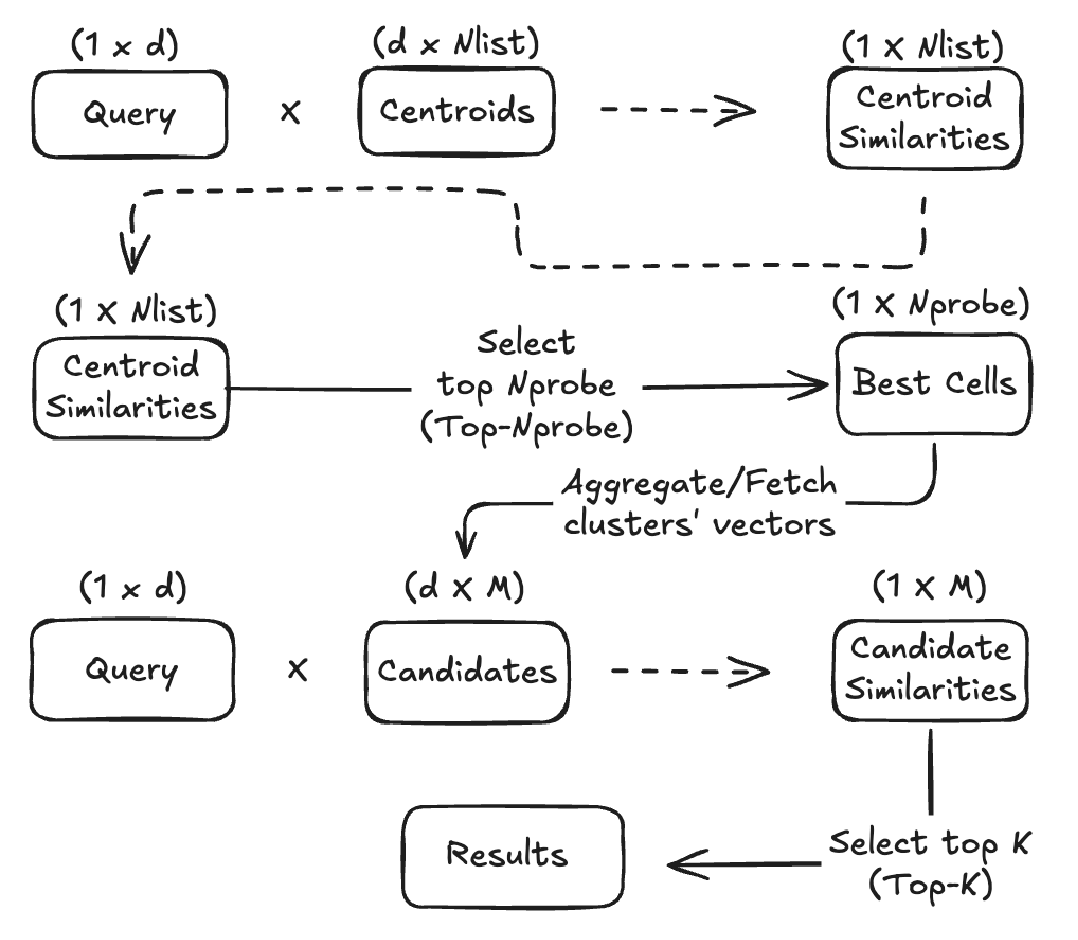
\includegraphics[width=0.90\textwidth]{./assets/ivf_search_pipeline.png}
\caption{Logical IVF-Flat query-processing pipeline. The query is first compared with all \(N_{\mathrm{list}}\) centroids. The \(N_{\mathrm{probe}}\) best cells are selected, their vectors define the candidate set, and the final top-\(k\) results are selected from the candidate similarities.}
\label{fig:ivf-search-pipeline}
\end{figure}

The figure is intentionally logical rather than physical: selected candidates are not copied into a single temporary matrix. Instead, database vectors remain grouped by inverted list in device memory and are streamed directly from the selected complete lists during fine search.

Queries are represented internally in groups containing between one and 32 valid queries, matching the row dimension of the \(32\times32\) tile representation used by the Tensix compute kernels. A group containing fewer than 32 valid queries is completed with zero-valued padded rows. For a workload containing \(Q\) valid queries, the implementation uses
\begin{equation}
B=\left\lceil\frac{Q}{32}\right\rceil
\end{equation}
internal query batches. The final batch is padded when \(Q\) is not divisible by 32. The number of valid rows is retained separately, so padded rows do not participate in coarse-result processing and do not contribute inverted lists to the fine-search schedule. They are also discarded when the final results are converted back to the host representation.

Although the implementation is described throughout the chapter in terms of one 32-query batch for clarity, the final system can process multiple such batches within one coarse-search and one fine-search invocation. The transition from the initial single-batch implementation to this multi-batch design is discussed in Section~\ref{sec:multi-batch-execution}.

\subsection{Host--Device Work Partitioning}
\label{subsec:host-device-responsibilities}

The index data required by both search stages remain resident on the Tenstorrent device across query workloads, including the centroid matrix, database vectors grouped by inverted list, and the corresponding original vector identifiers. In contrast, query-dependent data, such as the query buffer, coarse-search outputs, selected-list metadata, worker schedules, partial results, and final outputs, are updated for each search workload.

A synchronization boundary separates the coarse and fine programs. After the device executes coarse search and returns a fixed-size set of centroid candidates for each valid query, the host performs the final \(N_{\mathrm{probe}}\) selection, obtains the offset and padded length of each corresponding complete inverted list, groups the selected work at batch granularity, and constructs the per-worker fine-search descriptions. Only once this query-dependent schedule has been prepared is the fine-search program launched.

Figure~\ref{fig:host-device-pipeline} shows the division of responsibilities between the host and the device, together with the synchronization boundary between coarse and fine search.

\begin{figure}[htbp]
\centering
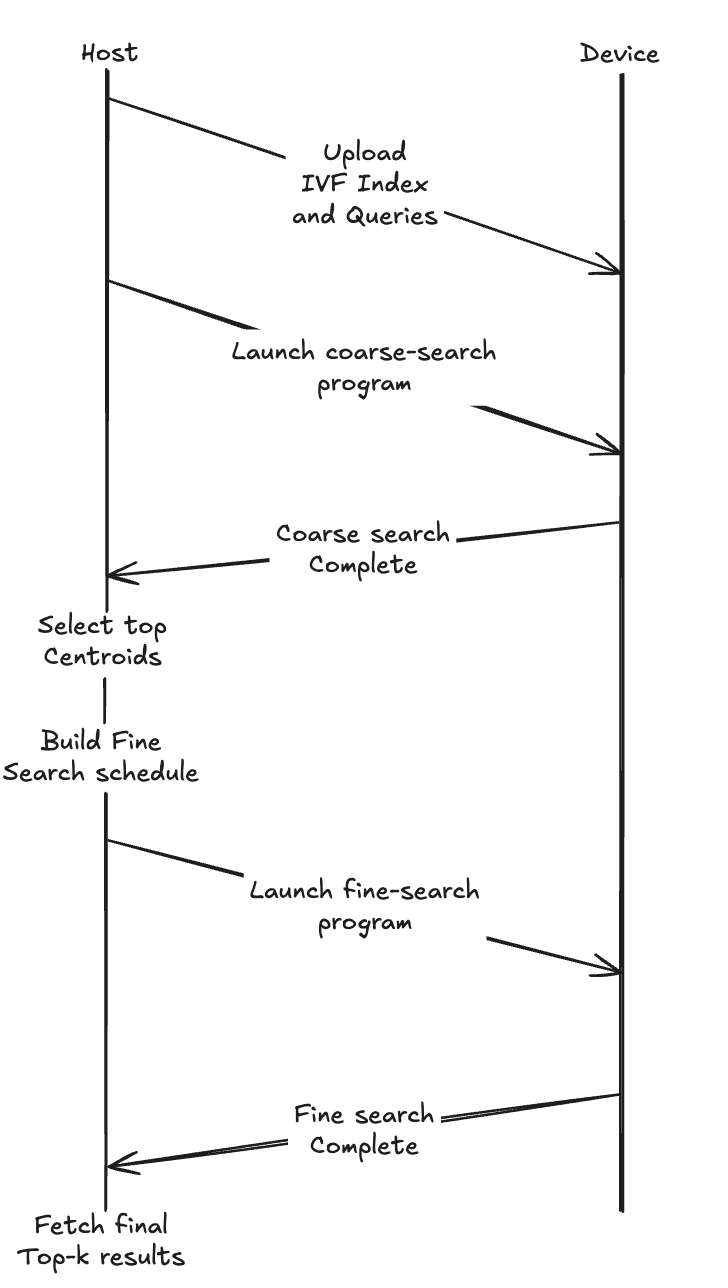
\includegraphics[width=0.80\textwidth]{./assets/host_device_pipeline.png}
\caption{Host--device interaction during one IVF search workload. The host loads the IVF index and query batch, launches the coarse-search program, receives the coarse-search results, selects the \(N_{\mathrm{probe}}\) lists and builds the fine-search schedule, then launches the fine-search program and fetches the final top-\(k\) results.}
\label{fig:host-device-pipeline}
\end{figure}

Each device program is decomposed into \emph{reader}, \emph{compute}, and \emph{writer} kernels connected through circular buffers, allowing data movement and computation to overlap when dependencies and buffer capacity permit it. Throughout this chapter, reader, compute, and writer denote kernels executing on a Tensix core, whereas worker and aggregation core denote logical roles assigned to complete Tensix cores. The terms \emph{coarse phase} and \emph{fine phase} refer to complete TT-Metalium programs rather than to individual kernels.

\section{Device-Oriented IVF Representation}
\label{sec:device-oriented-ivf}

\subsection{Index Construction}
\label{subsec:index-construction}

Index training is treated as an offline preprocessing step and is outside the timed search path. A representative subset of the database vectors is clustered with Faiss \(k\)-means to obtain \(N_{\mathrm{list}}\) centroids \cite{faiss}, following the same training procedure used by the CPU and GPU baselines based on Faiss \texttt{IndexIVFFlat}. The trained centroid matrix is exported and reused by the Tenstorrent implementation. Reusing the same centroids avoids making index-training quality an additional experimental variable and allows the evaluation to focus on differences in search execution.

Training is not performed on the Tenstorrent device because the objective of this work is the online IVF search path rather than accelerator-based \(k\)-means. An on-device training implementation would require additional iterative kernels for vector assignment, per-cluster accumulation, centroid normalisation, and convergence control, together with temporary device-memory capacity for the intermediate state. Those operations would neither be part of the measured query path nor improve the fairness of the search comparison. During construction of the Tenstorrent-oriented index, each database vector is assigned to its closest exported centroid and placed in the corresponding packed inverted list.

The Tenstorrent index stores full, uncompressed database vectors rather than compressed representations. Database vectors and centroids are normalised before assignment and search, allowing inner product to be used as the similarity measure.

Because the resulting inverted lists are not guaranteed to have equal sizes, assigning the same number of lists to every core does not necessarily assign the same amount of work. The fine-search scheduler therefore reasons about the number of 32-vector pages contained in each selected list rather than only the number of lists.

\subsection{Tiled Data Layout and Memory Placement}
\label{subsec:tiled-list-layout}

As introduced in Chapter~\ref{chap:background}, Tensix computation is organised around \(32\times32\) tiles \cite{tenstorrent_metalium_architecture}. Let \(D\) denote the original vector dimension. To match this tile-oriented execution model, the dimension is padded to
\begin{equation}
D_{\mathrm{p}}=32\left\lceil\frac{D}{32}\right\rceil.
\label{eq:dimension-padding}
\end{equation}
All values introduced by dimensional padding are set to zero on the host before the data are transferred to the device.

Vectors assigned to the same inverted list are stored consecutively in one logical packed database buffer. For a list containing \(L_j\) valid vectors, its stored length is rounded to a multiple of 32:
\begin{equation}
L_{j,\mathrm{p}}=32\left\lceil\frac{L_j}{32}\right\rceil.
\label{eq:list-padding}
\end{equation}
Each group of 32 vectors forms one \emph{candidate page}. A page contains \(D_{\mathrm{p}}/32\) 16-bit floating-point (\texttt{FP16}) data tiles, each of shape \(32\times32\), which together represent the 32 candidate vectors over the complete padded dimension. Centroids and queries use the same \texttt{FP16} representation, while vector identifiers are stored as 32-bit unsigned integers (\texttt{UInt32}). The Tenstorrent compute configuration enables FP32 destination accumulation. This mode is required by the employed top-\(k\) path when score tiles are ordered together with \texttt{UInt32} identifier tiles.

A candidate page must not be confused with a query batch. A query batch contains up to 32 queries and forms the row operand of fine search, whereas a candidate page contains 32 database vectors and forms the column operand. Their matrix product evaluates every query in the batch against every vector in the page. Figure~\ref{fig:pedagogical-batch-page} illustrates this distinction with a \(4\times4\) example.

\begin{figure}[htbp]
\centering
\resizebox{0.98\textwidth}{!}{%
\begin{tikzpicture}[font=\small]
\node[draw,rounded corners,fill=blue!8,inner sep=7pt] (queries) {$
Q_b=
\begin{bmatrix}
q_0^{\mathsf T}\\
q_1^{\mathsf T}\\
q_2^{\mathsf T}\\
q_3^{\mathsf T}
\end{bmatrix}_{4\times D_{\mathrm p}}
$};
\node[draw,rounded corners,fill=green!9,inner sep=7pt,
      right=1.2cm of queries] (page) {$
V_p=
\begin{bmatrix}
\vert&\vert&\vert&\vert\\[-2pt]
v_0&v_1&v_2&v_3\\[-2pt]
\vert&\vert&\vert&\vert
\end{bmatrix}_{D_{\mathrm p}\times4}
$};
\node[draw,rounded corners,fill=orange!12,inner sep=7pt,
      right=1.2cm of page] (scores) {$
S_{b,p}=
\begin{bmatrix}
s_{00}&s_{01}&s_{02}&s_{03}\\
s_{10}&s_{11}&s_{12}&s_{13}\\
s_{20}&s_{21}&s_{22}&s_{23}\\
s_{30}&s_{31}&s_{32}&s_{33}
\end{bmatrix}
$};
\node at ($(queries.east)!0.5!(page.west)$) {$\times$};
\node at ($(page.east)!0.5!(scores.west)$) {$=$};
\node[below=3pt of queries,font=\scriptsize] {query batch};
\node[below=3pt of page,font=\scriptsize] {candidate page};
\node[below=3pt of scores,font=\scriptsize] {query--candidate scores};
\end{tikzpicture}
}
\caption{Pedagogical \(4\times4\) example of one fine-search matrix
multiplication. Rows represent queries and columns represent candidate vectors.
The implementation uses \(32\times32\) tiles rather than the reduced size
shown here.}
\label{fig:pedagogical-batch-page}
\end{figure}

For every candidate page, one full \(32\times32\) \texttt{UInt32} identifier tile is stored. In its DRAM representation, each column corresponds to one candidate vector and the same 32 identifiers are replicated across all query rows. For candidate identifiers \(i_0,\ldots,i_{31}\), the stored tile is
\begin{equation}
I^{\mathrm{stored}}=
\begin{bmatrix}
i_0 & i_1 & \cdots & i_{31}\\
i_0 & i_1 & \cdots & i_{31}\\
\vdots & \vdots & \ddots & \vdots\\
i_0 & i_1 & \cdots & i_{31}
\end{bmatrix}.
\label{eq:identifier-tile}
\end{equation}
Before the compute-kernel \texttt{topk\_local\_sort} operation, both the similarity tile and its companion identifier tile are transposed. The identifier tile presented to the selection operation is therefore
\begin{equation}
I^{\mathrm{topk}}
=
\left(I^{\mathrm{stored}}\right)^{\mathsf T}
=
\begin{bmatrix}
i_0 & i_0 & \cdots & i_0\\
i_1 & i_1 & \cdots & i_1\\
\vdots & \vdots & \ddots & \vdots\\
i_{31} & i_{31} & \cdots & i_{31}
\end{bmatrix}.
\label{eq:identifier-tile-topk}
\end{equation}
After transposition, each column corresponds to one query and the rows represent candidate entries. The \texttt{topk\_local\_sort} operation sorts candidate entries independently for each query column. Applying the same transpose and ordering operations to the score and identifier tiles preserves the association between every similarity value and its original database-vector identifier. This transpose-and-sort mechanism is used by both coarse and fine search whenever a running top-32 score and identifier state is updated.

The vectors of all inverted lists are stored sequentially in a single packed device buffer. Each inverted list is identified by its offset within this buffer and by its length, rather than being stored in a separate device allocation. Vector identifiers occupy a separate packed \texttt{UInt32} buffer using the same list and page ordering. An inverted-list offset therefore identifies a position in this global logical representation. At the physical memory level, TT-Metalium interleaves buffer pages across DRAM banks, so ``contiguous'' refers to the logical buffer layout rather than to consecutive bytes within one DRAM bank.

Persistent search data are allocated in device DRAM, including the centroid matrix, packed database-vector buffer, and packed vector-identifier buffer. Query buffers and worker descriptions are likewise allocated in DRAM for each search workload, while per-core L1 memory is used as transient kernel-local storage through circular buffers. During execution, data required by the active kernels are streamed from DRAM into L1 rather than persistently cached across search invocations. The exact reuse and streaming strategy of the coarse- and fine-search programs is described in Sections~\ref{sec:coarse-search} and~\ref{subsec:fine-worker-pipeline}, respectively.
\newline
Padding is performed entirely on the host before device transfer:
\begin{itemize}
    \item database dimensional padding and inverted-list length padding are generated during \texttt{IVF\_TT::create\_index}.
    \item centroid dimensional padding is generated while constructing the centroid buffer in \texttt{load\_to\_device}.
    \item query dimensional padding and final-batch row padding are generated in \texttt{search\_all}.
\end{itemize}
Padded vector identifiers are assigned the sentinel value \texttt{0xffffffff} on the host.

Padded candidate positions contain zero-valued vectors and carry the sentinel identifiers defined above. Before local top-\(k\) selection, the fine-search compute kernel linearly scans the score and identifier entries of the final partially populated page of each inverted list. Whenever a sentinel identifier is encountered, the corresponding similarity value is replaced with \(-10000\), preventing padded candidates from displacing valid results during selection. The database and query vectors are normalised, so a valid inner product is bounded below by \(-1\) in exact arithmetic; \(-10000\) is therefore safely outside the valid similarity range. Complete candidate pages contain 32 valid vectors and bypass this masking step, avoiding an unnecessary scan of all \(32\times32=1024\) entries when no padding is present.

\section{Coarse Search}
\label{sec:coarse-search}

The purpose of coarse search is to identify the inverted lists most relevant to each query. For a valid query batch \(Q_b\in\mathbb{R}^{32\times D_{\mathrm{p}}}\) and centroid matrix \(C\in\mathbb{R}^{D_{\mathrm{p}}\times N_{\mathrm{list}}}\), the logical operation is
\begin{equation}
S^{\mathrm{coarse}}_b=Q_bC,
\label{eq:coarse-search}
\end{equation}
where each row of \(S^{\mathrm{coarse}}_b\) contains the similarities between one query and all centroids.

Tiling proceeds over blocks of 32 centroids. After loading the query batch from DRAM into an L1 circular buffer, the reader kernel streams centroid blocks from device DRAM while retaining the query for reuse across the complete centroid matrix. Let \(C_c\in\mathbb{R}^{D_{\mathrm{p}}\times32}\) denote centroid block \(c\).

The corresponding coarse-similarity tile is
\begin{equation}
S^{\mathrm{coarse}}_{b,c}=Q_bC_c,
\qquad
S^{\mathrm{coarse}}_{b,c}\in\mathbb{R}^{32\times32}.
\label{eq:coarse-similarity-tile}
\end{equation}
Rather than materialising all \(N_{\mathrm{list}}\) similarities in DRAM, the compute kernel incrementally maintains the 32 highest centroid scores and their identifiers for each query row. This running top-32 state uses the same transpose-and-\texttt{topk\_local\_sort} mechanism described in Section~\ref{subsec:tiled-list-layout}, with identical ordering decisions applied to scores and centroid identifiers.

Once all centroid blocks assigned to a query batch have been processed, the coarse-search writer kernel running on the same participating Tensix core writes one score tile and one identifier tile for that batch to device DRAM. After copying these results to the host, the host orders and deduplicates the valid centroid identifiers and retains the first \(N_{\mathrm{probe}}\) lists for each query. Consequently, the current implementation limits \(N_{\mathrm{probe}}\) to at most 32.

Multiple query batches are distributed by the coarse-search program across the available participating cores, with each active core processing one or more complete batches and avoiding inter-core communication during the centroid scan. Because every valid query is evaluated against the same centroid matrix, coarse search remains regular and requires a predictable amount of work.

\section{Fine-Search Scheduling}
\label{sec:fine-search-scheduling}

Fine search introduces the principal source of irregularity in the system. Every valid query selects the same number \(N_{\mathrm{probe}}\) of inverted lists, but the identifiers and lengths of those lists depend on the query. Two queries with the same \(N_{\mathrm{probe}}\) may therefore require very different amounts of candidate processing. The imbalance remains after lists are combined at batch level: one worker assigned several short lists can finish before another worker assigned one very long list.

The scheduler estimates the cost of a selected list by its number of padded 32-vector candidate pages. This page count is used only as a scheduling weight: an inverted list remains an indivisible task and is never partitioned into page ranges shared by multiple workers.

\subsection{Batch-Level List Union}
\label{subsec:batch-level-union}

After coarse search, each query row has up to \(N_{\mathrm{probe}}\) selected inverted-list identifiers. Since fine search operates on a complete batch of up to 32 queries, the host collects these identifiers into a single set of lists for the batch.

Let \(\mathcal{P}_{b,r}\) denote the \(N_{\mathrm{probe}}\) lists selected for query row \(r\) of batch \(b\). The set of lists processed for the batch is
\begin{equation}
\mathcal{U}_b
=
\bigcup_{r\in\mathcal{V}_b}
\mathcal{P}_{b,r},
\label{eq:batch-union}
\end{equation}
where \(\mathcal{V}_b\) contains the valid query rows of the batch.

Operationally, the host iterates over the coarse-search results of every valid query row and inserts the first \(N_{\mathrm{probe}}\) list identifiers into a set. Duplicate identifiers are therefore automatically removed. The resulting set \(\mathcal{U}_b\) contains every inverted list selected by at least one query in the batch.

The batch-level union is motivated by the execution granularity of the Tensix matrix engine. Fine search operates on \(32\times32\) tiles: one candidate page contains 32 vectors, while one query tile contains up to 32 queries. For a candidate page \(V_p\), the device evaluates
\begin{equation}
Q_bV_p,
\qquad
Q_b\in\mathbb{R}^{32\times D_{\mathrm{p}}},
\qquad
V_p\in\mathbb{R}^{D_{\mathrm{p}}\times32},
\end{equation}
producing a \(32\times32\) similarity tile.

Because Tensix executes the matrix multiplication at tile granularity, processing a candidate page for only one query row does not reduce the cost of the matrix operation relative to processing it for the complete query tile. A computation conceptually involving a \(1\times D_{\mathrm{p}}\) query would still occupy the same tiled execution unit after padding to the required representation. Therefore, once a candidate page is selected for processing, evaluating it against the remaining queries of the batch does not require an additional matrix multiplication.

As a consequence, a query can also obtain similarity scores for vectors belonging to a list that was selected by another query in the same batch. The effective candidate set for one query can therefore be larger than the set defined by its own \(N_{\mathrm{probe}}\) lists. This is an implementation consequence of processing the batch-level union and does not modify the stored IVF index.

The union can nevertheless increase the total amount of fine-search work because lists selected by different queries may not overlap, increasing the number of distinct candidate pages that must be processed. The benefit of the design therefore comes from fully exploiting each tile-level matrix multiplication, rather than from making the additional lists computationally free.

\subsection{Greedy Work Distribution}
\label{subsec:greedy-work-distribution}

For each list \(j\in\mathcal{U}_b\), the host creates one indivisible task that covers the entire inverted list. Its scheduling weight is the number of padded candidate pages in that list, \begin{equation} p_j=\left\lceil\frac{L_j}{32}\right\rceil, \label{eq:list-scheduling-weight} \end{equation} where \(L_j\) is the number of valid vectors in list \(j\). Thus, for example, lists containing 320 and 288 vectors have weights 10 and 9, respectively. These weights count the fixed-shape page multiplications expected for each list; they are not fractions used to divide a list among workers.

The implementation configures an \(8\times8\) logical grid of 64 Tensix cores. Logical core \((0,0)\) is reserved for final aggregation, and all remaining 63 cores form the fine-search worker set \(\mathcal{W}\). For every query batch, let \(\mathcal{A}_{b,w}\) denote the lists assigned to worker \(w\). The scheduler resets both the assignments and their estimated loads,
\begin{equation}
\mathcal{A}_{b,w}=\varnothing,
\qquad
\lambda_{b,w}=0,
\qquad w\in\mathcal{W},
\end{equation}
sorts the tasks in non-increasing order of \(p_j\), and assigns each complete list to a currently least-loaded worker:
\begin{align}
w^*&=\arg\min_{w\in\mathcal{W}}\lambda_{b,w},\\
\mathcal{A}_{b,w^*}&\leftarrow\mathcal{A}_{b,w^*}\cup\{j\},\\
\lambda_{b,w^*}&\leftarrow\lambda_{b,w^*}+p_j.
\label{eq:greedy-list-assignment}
\end{align}
The secondary ordering key for equal page counts is ascending inverted-list identifier. If several workers have the same minimum load, the worker with the lowest index is selected. These explicit tie rules make the host schedule reproducible. The resulting longest-task-first greedy policy attempts to balance the padded page count while retaining sequential access within every packed list.

Figure~\ref{fig:pedagogical-list-scheduling} shows the process for a reduced four-query example. The displayed values 10, 9, 6, and 4 are page-count weights. In particular, a list of weight 10 remains one task; it is not split into ten independently assignable ranges.

\begin{figure}[htbp]
\centering
\begin{tikzpicture}[font=\small,>=Latex]
\node[draw,rounded corners,fill=blue!8,align=left,text width=3.25cm,
      inner sep=7pt] (selected) at (-4.15,0) {
\textbf{Selections}\par
\(q_0:\{A,B\}\)\par
\(q_1:\{A,C\}\)\par
\(q_2:\{B,D\}\)\par
\(q_3:\{A,D\}\)};

\node[draw,rounded corners,fill=orange!10,align=left,text width=3.25cm,
      inner sep=7pt] (union) at (0,0) {
\textbf{Batch union}\par
\(\mathcal U_b=\{A,B,C,D\}\)\par
\(p_A=10,\ p_B=9\)\par
\(p_C=6,\ p_D=4\)};

\node[draw,rounded corners,fill=green!9,align=left,text width=3.25cm,
      inner sep=7pt] (workers) at (4.15,0) {
\textbf{Greedy assignment}\par
\(w_0:\{A\},\ \lambda=10\)\par
\(w_1:\{B\},\ \lambda=9\)\par
\(w_2:\{C,D\},\ \lambda=10\)};

\draw[-{Latex[length=2mm]}] (selected.east) -- (union.west);
\draw[-{Latex[length=2mm]}] (union.east) -- (workers.west);
\end{tikzpicture}
\caption{Pedagogical four-query example of batch-level list union and greedy
whole-list scheduling. The real implementation uses batches of up to 32
queries and all configured fine-search workers. Each selected list is an
indivisible task weighted by its padded number of candidate pages.}
\label{fig:pedagogical-list-scheduling}
\end{figure}

The page count is an estimate rather than a cycle-accurate cost model. It does not capture per-list setup, masking of the final partial page, variation in memory service time, circular-buffer waiting, or synchronization. Moreover, because a large inverted list cannot be divided, the longest list can still determine the batch completion time. After scheduling, the host serialises one description per fine-search worker so that its reader kernel can locate the assigned complete lists in device memory.

\subsection{Worker Description}
\label{subsec:worker-description}

The host serialises the fine-search assignment into one logical flattened worker description in DRAM for each fine-search worker. A description can span multiple DRAM pages, so it is not restricted to one physical page. It contains the information required by the reader kernel to locate the query batches and the complete inverted lists assigned to that worker.

Let \(B\) denote the number of query batches, as introduced in Section~\ref{subsec:end-to-end-pipeline}. The worker description has the conceptual form
\begin{equation}
W_w
=
\left\langle
B,\,
R_0,\,
R_1,\,
\ldots,\,
R_{B-1}
\right\rangle,
\label{eq:worker-description}
\end{equation}
where \(R_b\) describes the work assigned to worker \(w\) for query batch \(b\).

Each batch record contains the global offset of the query batch in the query buffer, the number of tiles used to represent it, and the number of whole-list tasks that the worker must process:
\begin{equation}
R_b
=
\left\langle
o^{Q}_b,\,
n^{Q}_b,\,
N^{(w)}_{\mathrm{list},b},\,
E^{(w)}_{b,0},\,
E^{(w)}_{b,1},\,
\ldots,\,
E^{(w)}_{b,N^{(w)}_{\mathrm{list},b}-1}
\right\rangle,
\label{eq:worker-batch-record}
\end{equation}
where \(o^{Q}_b\) is the global offset of query batch \(b\) in the query buffer, \(n^{Q}_b\) is the number of tiles composing its padded representation, and \(N^{(w)}_{\mathrm{list},b}\) is the number of whole-list tasks assigned to worker \(w\) for that batch.

Each whole-list entry \(r\) is represented as
\begin{equation}
E^{(w)}_{b,r}
=
\left\langle
o^{V}_{b,r},\,
n^{V}_{b,r}
\right\rangle,
\label{eq:worker-list-record}
\end{equation}
where \(o^{V}_{b,r}\) is the global candidate-page offset of the assigned inverted list in the packed database buffer, and \(n^{V}_{b,r}\) is the number of candidate pages in that complete list. Although the record is encoded as an offset and page-count pair, it always describes an entire selected list; the scheduler does not create subranges. Since each candidate page contains 32 vectors, these two values are sufficient for the reader kernel to determine where the list begins and how many candidate-vector and identifier tiles must be fetched from their respective packed buffers.

At the beginning of fine search, each worker copies its description from DRAM into local L1. For each batch with assigned work, the corresponding query tiles are loaded once into the local query circular buffer and remain resident while all whole-list tasks associated with that batch are processed. The reader then advances to the next batch record and repeats the same procedure.

\section{Fine Search and Result Reduction}
\label{sec:fine-search-and-reduction}

\subsection{Worker Pipeline}
\label{subsec:fine-worker-pipeline}

The fine-search program evaluates the candidate pages selected by the host schedule. As defined above, logical core \((0,0)\) performs final aggregation, while the other 63 cores in the configured \(8\times8\) logical grid operate as fine-search workers.

Each worker executes reader, compute, and writer kernels concurrently. At the beginning of the invocation, the reader loads the worker description from DRAM into local L1; for each active query batch, the query tiles are then loaded once into the worker's query circular buffer and retained while all candidate pages assigned to that worker for the batch are processed.

Candidate vectors and their identifier tiles are streamed from the packed DRAM buffers. The reader issues both reads before a shared synchronization barrier, allowing their transfers over the on-device Network-on-Chip (NoC) to be outstanding concurrently. Double-buffering of the candidate circular buffers allows the reader to prepare a later page while the compute kernel operates on an earlier one, subject to circular-buffer capacity and producer--consumer synchronization.

Let \(j\) identify a whole inverted-list task assigned to the worker and let \(p\) identify a candidate page within that list. For one such page \(V_{j,p}\in\mathbb{R}^{D_{\mathrm{p}}\times32}\), the compute kernel evaluates
\begin{equation}
S^{\mathrm{fine}}_{b,j,p}=Q_bV_{j,p},
\label{eq:fine-search}
\end{equation}
producing a \(32\times32\) tile of query--candidate similarities.

Across all candidate pages assigned to it, the worker incrementally maintains a row-wise top-32 state, with scores and original vector identifiers propagated together through the same ordering operations. No list-local to global identifier reconstruction is therefore required after the search.

Figure~\ref{fig:fine-local-topk} shows the local top-32 update performed by one fine-search worker. Two \(32\times32\) tiles hold the best scores and identifiers found so far, while the other two contain the scores and identifiers of the current candidate page. Before selection, the current and saved score and identifier tiles are transposed so that each column corresponds to one query and the rows contain candidate entries. The compute-kernel \texttt{topk\_local\_sort} operation then applies the same ordering decisions to the score and identifier tiles, preserving the association between every similarity value and its original vector identifier.

\begin{figure}[htbp]
\centering
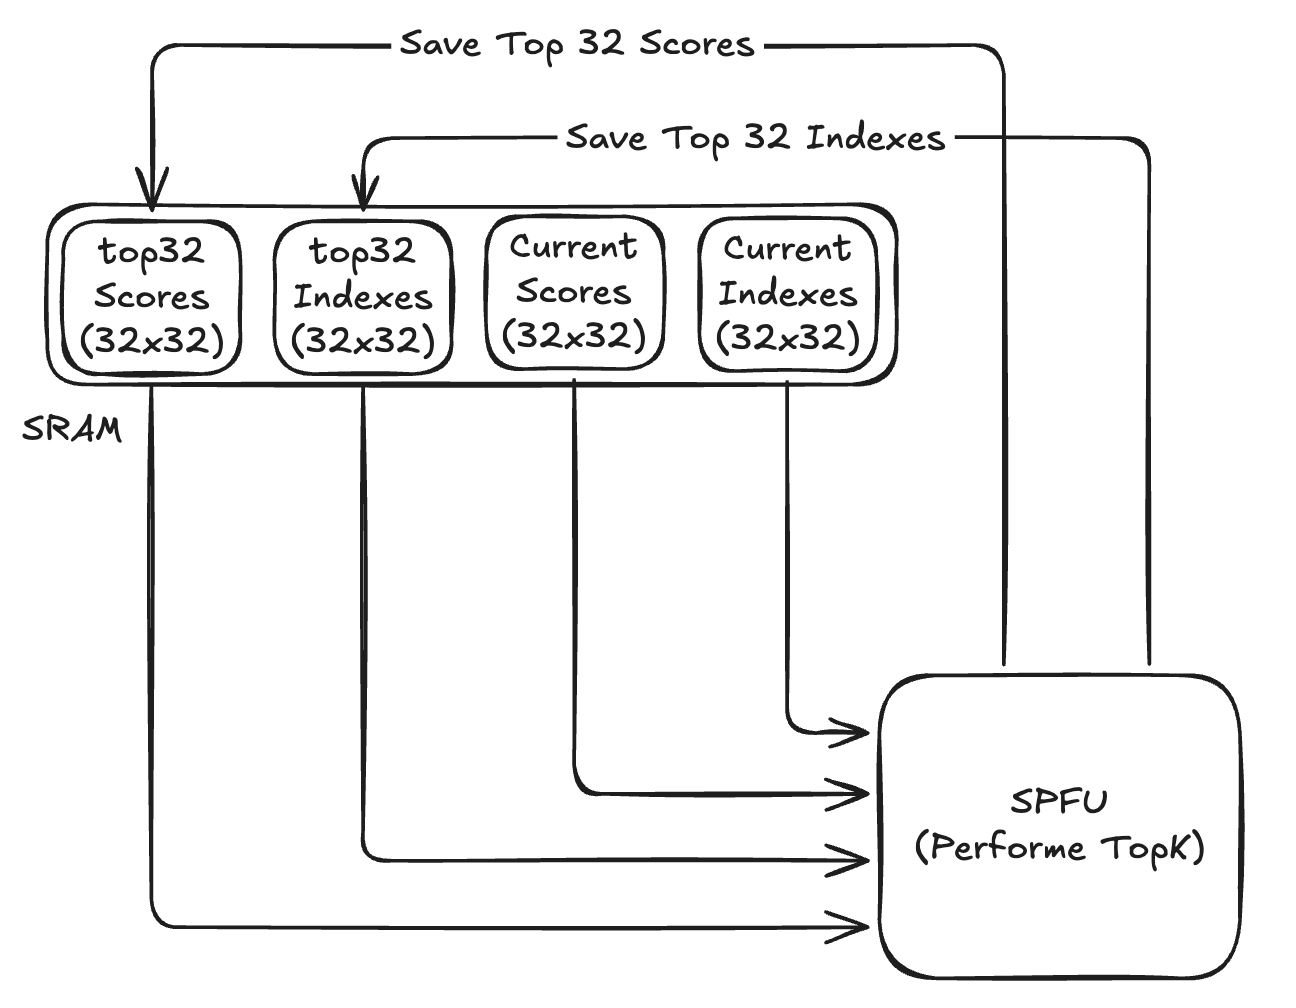
\includegraphics[width=0.78\textwidth]{./assets/fine_search_local_topk.png}
\caption{Worker-local top-32 update. Before selection, the score and identifier tiles are transposed so that each column corresponds to one query and the rows contain candidate entries from the saved and current states. The \texttt{topk\_local\_sort} operation applies identical ordering decisions to scores and identifiers.}
\label{fig:fine-local-topk}
\end{figure}

\subsection{Hierarchical Top-\texorpdfstring{\(k\)}{k}}
\label{subsec:hierarchical-topk}

A single worker observes only part of the candidate set, so the final result is computed hierarchically. For query row \(r\) in batch \(b\), worker \(w\) first retains
\begin{equation}
R_{b,w,r}=\operatorname{Top}_{32}\left(\mathcal{C}_{b,w,r}\right),
\label{eq:worker-top32}
\end{equation}
where \(\mathcal{C}_{b,w,r}\) is the set of candidates evaluated by that worker.

Worker-local results are staged in DRAM, with each configured worker writing one fixed-size score tile and one identifier tile per query batch to a region indexed by batch and worker. All configured workers produce and signal one partial result for every batch, even when a worker has no active list task for that batch. In that case, every score remains at the initial value \(-10000\) and every identifier remains at \texttt{0xffffffff}.

Synchronization uses a cumulative completion semaphore in the L1 memory of logical core \((0,0)\). After writing its partial result for a batch, each worker increments this semaphore, and the aggregation reader waits until the expected number of increments has been observed. Once the partial result of a worker has been consumed, the aggregation reader increments a worker-specific ready semaphore in that worker's L1 memory, allowing the worker to reuse its partial-result slot and advance to the next batch.

Figure~\ref{fig:fine-partial-staging} illustrates this two-way handshake. Fine-search workers write their local top-32 results to distinct locations in the shared DRAM partial-result buffer and signal completion to the aggregation core; after consuming those results, core \((0,0)\) signals the corresponding workers that their slots can be reused.

\begin{figure}[htbp]
\centering
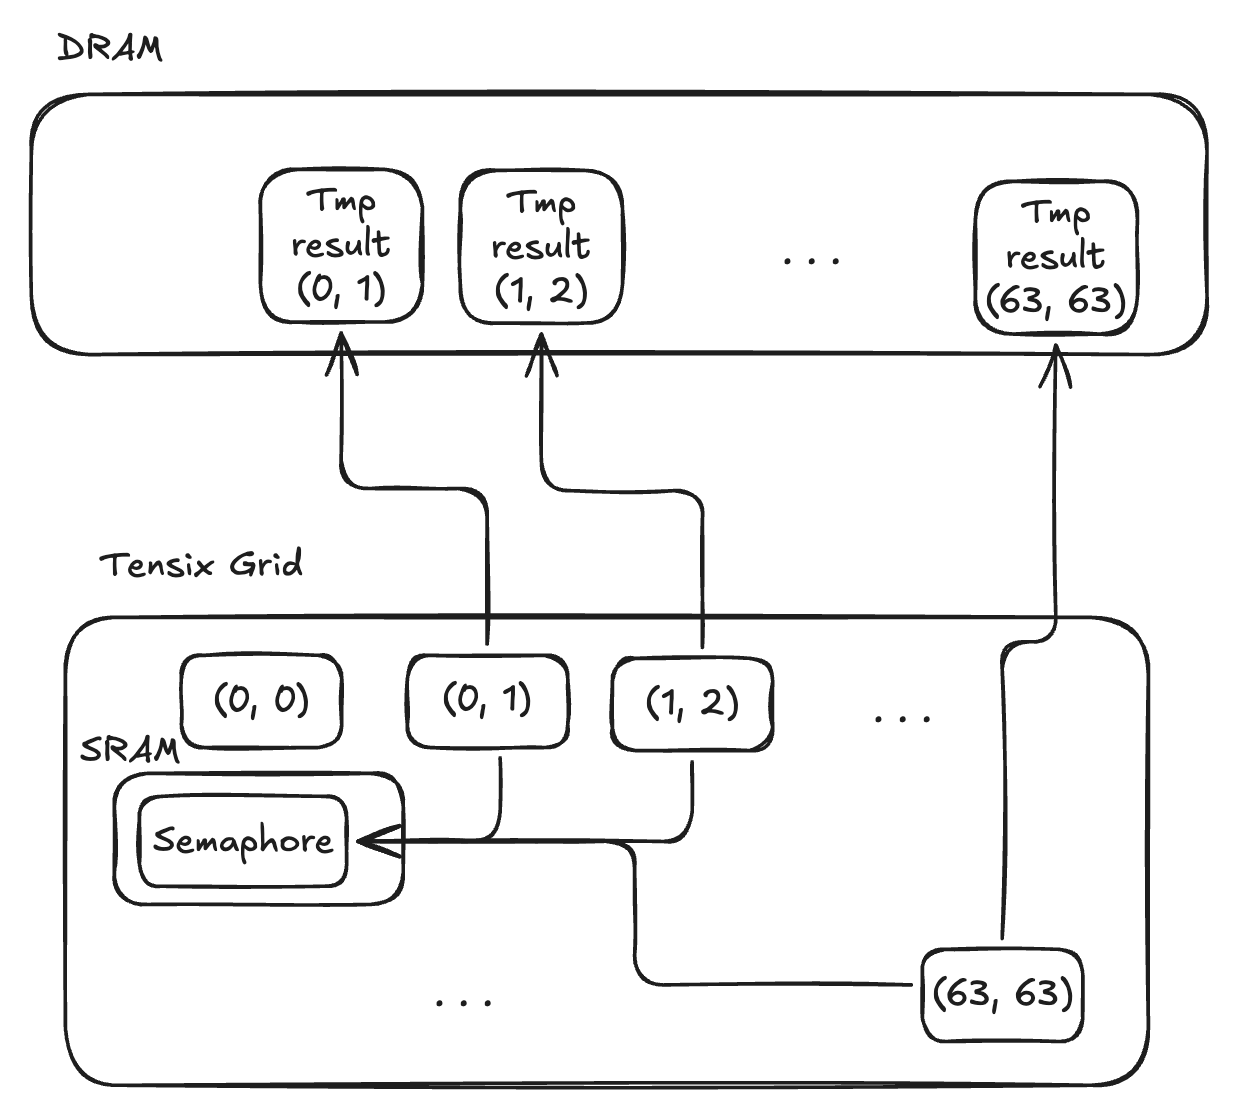
\includegraphics[width=0.78\textwidth]{./assets/fine_search_partial_results.png}
\caption{DRAM staging and synchronization of fine-search partial results. Workers store their local top-32 results in DRAM and synchronize with the aggregation core through completion and ready semaphores.}
\label{fig:fine-partial-staging}
\end{figure}

The aggregation compute kernel performs the second reduction,
\begin{equation}
R_{b,r}=\operatorname{Top}_{32}\left(\bigcup_w R_{b,w,r}\right),
\label{eq:global-top32}
\end{equation} and writes one final score tile and one final identifier tile per batch to DRAM. Figure~\ref{fig:pedagogical-hierarchical-topk} reduces the tile width from 32 to 4 to illustrate the two-level selection without the visual complexity of the actual result tiles.

\begin{figure}[htbp]
\centering
\begin{tikzpicture}[font=\small,>=Latex]
\node[draw,rounded corners,fill=blue!8,align=center,text width=2.65cm]
  (w0) at (-4.25,1.45) {worker 0\\local top-4};
\node[draw,rounded corners,fill=blue!8,align=center,text width=2.65cm]
  (w1) at (-4.25,0) {worker 1\\local top-4};
\node[draw,rounded corners,fill=blue!8,align=center,text width=2.65cm]
  (w2) at (-4.25,-1.45) {worker 2\\local top-4};

\node[draw,rounded corners,fill=orange!10,align=center,text width=2.8cm,
      minimum height=1.35cm] (merge) at (0,0)
  {aggregation core\\merge 12 candidates};
\node[draw,rounded corners,fill=green!10,align=center,text width=2.65cm,
      minimum height=1.35cm] (final) at (4.1,0)
  {global top-4\\for each query};

\draw[-{Latex[length=2mm]}] (w0.east) -- (merge.west);
\draw[-{Latex[length=2mm]}] (w1.east) -- (merge.west);
\draw[-{Latex[length=2mm]}] (w2.east) -- (merge.west);
\draw[-{Latex[length=2mm]}] (merge.east) -- (final.west);
\end{tikzpicture}
\caption{Pedagogical two-level result reduction for three workers, retaining
four entries. Each worker first retains its local best four candidates;
logical core \texttt{(0,0)} merges the partial results and retains the global
best four for each query. The implementation uses top-32 states and all
configured workers.}
\label{fig:pedagogical-hierarchical-topk}
\end{figure}

The host converts the tiled outputs to row-major form, removes sentinel entries, discards padded query rows, and retains the first \(k\) results for every valid query. The implementation therefore supports \(k\leq32\); the evaluation in this thesis uses \(k=10\).

For \(B\) query batches and \(W\) fine-search workers, logical core \((0,0)\) consumes \(BW\) worker-result pairs and performs \(BW\) running top-32 updates. Synchronization activity and partial-result traffic also grow linearly with the number of worker results. With \(W=63\), each batch contributes 63 score-and-identifier result pairs to the aggregation stage and requires 63 running top-32 updates. Because workers without active list tasks still write sentinel results, this cost depends on the configured worker count rather than the number of non-empty assignments. The centralised stage consequently scales as \(\Theta(BW)\) and can constrain designs with larger worker counts.

\section{Multi-Batch Execution}
\label{sec:multi-batch-execution}

The first implementation processed one batch of at most 32 queries per search invocation. This design matched the \(32\times32\) tile representation and simplified the initial implementation, but a larger query workload required the host to repeat query preparation, coarse execution, synchronization, list selection, fine-search scheduling, fine execution, final result transfer, and host-side orchestration for every group of 32 queries.

The final implementation, represented by \texttt{ann\_ivf\_dram\_args}, retains the same 32-query internal representation while allowing one search call to process multiple batches. After a coarse-search invocation processes all valid batches of the workload, the host constructs the fine-search descriptions for the complete set of selected lists. These logical descriptions may occupy multiple DRAM pages, so the format does not impose a fixed batch-count limit. The fine-search program then processes the paged descriptions within one larger invocation; practical capacity remains bounded by the device-memory allocation available to the workload.

This change separates tile size from execution granularity: a batch of 32 queries remains the natural unit of matrix computation, but it is no longer the unit at which the complete device pipeline must be launched. Repeated program configuration, launch, synchronization, and host orchestration are consequently amortised across a larger number of queries.

\section{Implementation Constraints}
\label{sec:implementation-constraints}

Table~\ref{tab:implementation-constraints} consolidates the implementation constraints derived in the preceding sections without repeating their full derivations.

\begin{table}[htbp]
\centering
\caption{Principal constraints of the evaluated Tenstorrent implementation.}
\label{tab:implementation-constraints}
\small
\setlength{\tabcolsep}{5pt}
\renewcommand{\arraystretch}{1.12}
\begin{tabularx}{\textwidth}{p{0.22\textwidth} p{0.31\textwidth} X}
\toprule
Constraint & Cause & Consequence \\
\midrule
Tile alignment
& The compute path operates on \(32\times32\) tiles.
& Vector dimensions and list lengths are padded to multiples of 32; an
  internal query batch contains up to 32 valid queries. \\

Centroid blocking
& Coarse search traverses complete 32-centroid blocks.
& The current representation requires \(N_{\mathrm{list}}\) to be divisible
  by 32. \\

Selection capacity
& Coarse, worker-local, and global selection use top-32 states.
& \(N_{\mathrm{probe}}\leq32\) and \(k\leq32\). The reported experiments use
  \(k=10\). \\

Whole-list scheduling
& A worker record addresses one complete inverted list.
& Lists cannot be split across workers, so a large list can determine the
  batch tail even after greedy balancing. \\

Paged worker descriptions
& A logical description may span multiple DRAM pages.
& The format imposes no fixed batch-count limit; practical capacity depends
  on the device-memory allocation available to the invocation. \\

Centralised reduction
& Every worker emits one partial result for every batch.
& Aggregation work and intermediate traffic scale as \(\Theta(BW)\), including
  sentinel results from workers with empty assignments. \\

Deployment scope
& The implementation targets one Wormhole n150 device.
& Multi-device approximate nearest-neighbour execution is outside the scope
  of this work. \\
\bottomrule
\end{tabularx}
\end{table}

Reader, compute, and writer kernels additionally share the local L1 capacity through their circular buffers, query tiles, intermediate similarities, identifier tiles, running top-32 states, and worker metadata. Buffer depth must therefore balance query reuse and double buffering against local-memory capacity. Progress also remains subject to circular-buffer backpressure, NoC completion, and the synchronization dependencies described above.

\section{Chapter Summary}
\label{sec:design-summary}

This chapter described the implementation of IVF-Flat search on a single-chip Tenstorrent Wormhole n150 device, with the index transformed into a tile-oriented representation in which vectors are grouped by inverted list and stored in 32-vector pages together with their original identifiers.

The search pipeline is divided into a regular coarse-search phase and an irregular fine-search phase. While coarse search reuses query tiles to scan the centroid matrix and return a fixed-size set of centroid candidates, the host subsequently selects the \(N_{\mathrm{probe}}\) lists, forms batch-level unions, and assigns complete selected lists to workers using their padded page counts as weights in a greedy longest-task-first scheduler.

Each fine-search worker reuses one query batch while streaming the candidate pages of its assigned lists and maintaining a worker-local row-wise top-32 state. The resulting partial results are staged in DRAM and merged on logical core \((0,0)\) before the final outputs are returned to the host.

The final design preserves the natural 32-query tile representation while extending execution to multiple batches per invocation. This reduces repeated host--device orchestration while preserving the same coarse- and fine-search stages and using batch-level list unions to match the tile-oriented execution model. The following chapter defines the methodology used to evaluate the resulting implementation.
